\documentclass[12pt, a4paper]{scrartcl}

\usepackage{a4wide}
\usepackage{graphicx}      
\usepackage{float}
\usepackage{amsmath}
\usepackage[
		colorlinks=false,
		urlcolor=blue,
		linkcolor=white
]{hyperref}
\usepackage{booktabs}
\usepackage[font=footnotesize,labelfont=bf]{caption}

\usepackage[utf8]{inputenc}
%\usepackage[T1]{fontenc}
\usepackage[ngerman]{babel}

\renewcommand*\rmdefault{cmss}

\newcommand{\sciv}[4]{#1=#2\cdot10^{#3}\ #4}

\begin{document}
	
	\thispagestyle{empty}
	\null\vspace{40mm}
	\begin{center}
		{
			\Large  Die Nutzung von Vakuumpumpen für\\ unterschiedliche Anwendungen aufgrund ihrer Funktionsweise,\\ 
			sowie die Mechanik der Evakuierung	
			\footnote{
				\noindent Versuch F71, ausgeführt am 24.4.17,
				Betreuer: Frederik Arand,
				kurze besondere Auswertung
			}
		}\\[15mm]
		P. Nisblé und D. Bubeck
		
		\vspace{25mm}
		
		\parbox{0.9\textwidth}{
			Abstract:    
			\small The abstract should preferentially be in English. Here we explain in a
			few lines (i) what was done, and (ii) what the results were.
		}
	\end{center}
	
	\vfill
	Als besondere Auswertung testiert: Datum, Unterschrift:
	\vspace{20mm}
	
	%% Rueckseite des Titelblatts leer. Bei einseitigem Druck entfernen
	\newpage  
	\null\thispagestyle{empty} 
	
	%\newpage     % Inhaltsverzeichnis, koennte man bei langer Version machen
	%\tableofcontents 
	
	\newpage
	
	\pagenumbering{arabic} %% start page 1 
	\section{Einleitung}
		Diese Reihe von Versuchen dienen zur Orientierung und Nutzung von Apparaturen die Evakuierung benötigen, sowie zur Verständnis der Vakuumtechnik und auch deren Grenzen. In geringem Maße auch der Sensibilisierung für zuvor unbekannte Fehlerquellen die in der Vakuumtechnik zu Fehlern führen können.\\\\
		Der komplette Versuch ist getrennt in 6 Teilversuche: \cite{skript}
		\begin{enumerate}
			\item Funktionsweise einer Drehschieberpumpe
			
				Beobachtung einer Drehschieberpumpe in Betrieb und Bestimmung des maximal erreichbaren Vakuums (nach Abb. \ref{fig:anord1})

			\item Abpumpen kondensierbarer Dämpfe
				
				Beobachtung der selben Drehschieberpumpe unter Abpumpen kondensierbarer Dämpfe und dem daraus resultierenden maximalen Vakuum (nach Abb. \ref{fig:anord2})

			\item Funktionsweise von Molekular- und Turbomolekularpumpe (TMP)
			
                Beobachtung einer Hybridpumpe mit Turbo- und Gaedestufe in Betrieb
                (nach Abb. \ref{fig:anord3})
			
			\item Saugvermögen der TMP
			
            	Messung des Saugvermögens der TMP mithilfe einer Kapillaren
                (nach Abb. \ref{fig:anord4})
			
			\item Bestimmung des Leitwerts von Rohr und Blende
            	
                (nach Abb. \ref{fig:anord5})
			
			\item Lecksuche
			
            	mit Teslatransformator und Heliumlecksucher
                (nach Abb. \ref{fig:anord6})
		\end{enumerate}
	\newpage
	\section{Versuchsdurchführung}
	\subsection{Inbetriebnahme der Drehschieberpumpe}
	
        \begin{figure}[H]
            \centering
            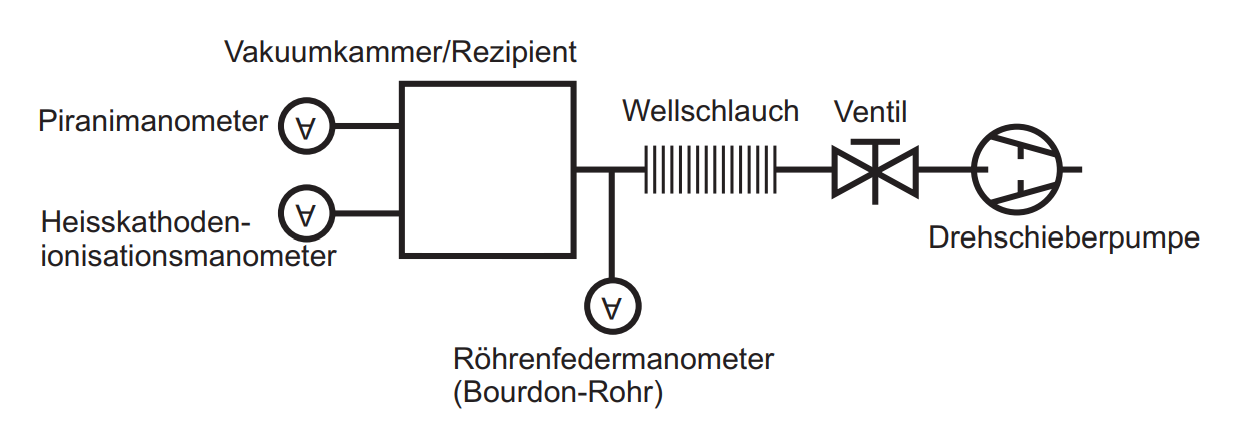
\includegraphics[width=.5\paperwidth]{aufbau21}
            \caption{generalisierter Aufbau zur Beobachtung der Funktionsweise einer Drehschieberpumpe}
            \label{fig:anord1}
        \end{figure}
    
    	
    	
    	Es hat sich ein Enddruck der Drehschieberpumpe bei \begin{align*}
            (1.2\pm 0.1)\cdot 10^{-1}\ mbar
        \end{align*}
        Aufgrund des zu großen Enddrucks und der darauffolgenden Lecksuche, welche neagtiv war, wird angenommen, dass sich noch Wasser im System befunden hat. (Versuchsteil 2 wurde vorgezogen)
    
    
    
    \subsection{Abpumpen kondensierbarer Dämpfe}
    
		\begin{figure}[H]
			\centering
			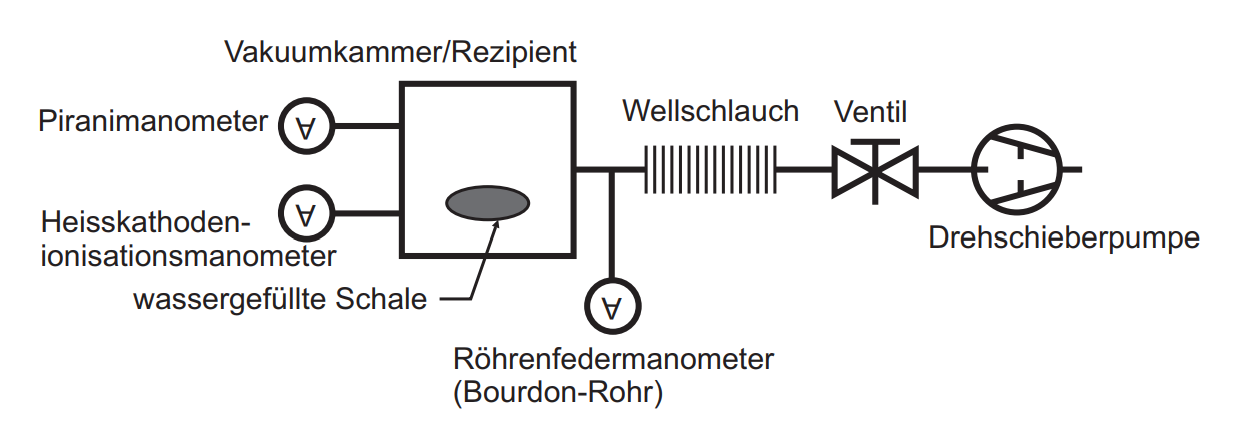
\includegraphics[width=.5\paperwidth]{aufbau22}
			\caption{Vakuum-Blockschaltbild zum Versuch des Abpumpens kondensierbarer Dämpfe}
            \label{fig:anord2}
		\end{figure}
	
		Beobachtung:
		\begin{itemize}
			\item Wasser beginnt bei niedrigem Druck an zu sieden
			
			$\rightarrow$ Schalte Gasballast zu um Kondensation des Wasserdampfes zu verhindern			
			
			\item Wasser gefriert bei $\sim 5.8\ mbar$
			
		\end{itemize}

	
	\subsection{Inbetriebnahme einer Turbomolekularpumpe}
	
        \begin{figure}[H]
            \centering
            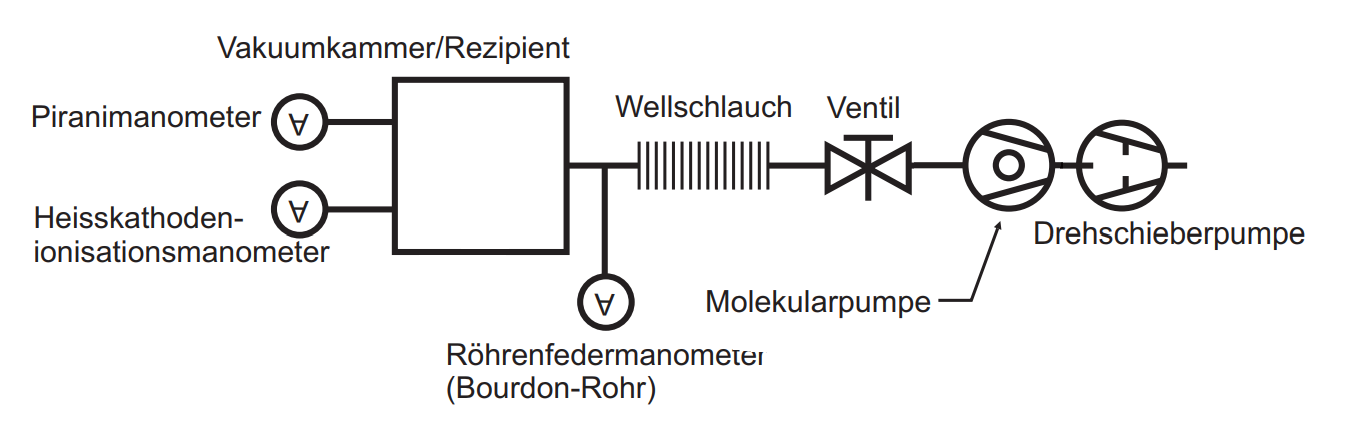
\includegraphics[width=.55\paperwidth]{aufbau23}
            \caption{Aufbau zur Beobachtung der Funktionsweise von Molekular- und Turbomolekularpumpe}
            \label{fig:anord3}
        \end{figure}
    
    	Die Turbomolekularpumpe wird nun nach \cite{skript}, wie in Aufbau \ref{fig:anord3} hinzugeschalten. Die Apparatur wurde eingeschaltet und über Nacht laufen gelassen.
    	
    	Über Nacht hat sich der Druck im Rezipienten auf 
        $(1.1\pm0.1)\cdot 10^{-6}\ mbar$
        eingestellt. (gemessen mit dem Dual-Gauge-Messgerät)
        
        Die Frequenz der Turbomolekularpumpe beträgt $f = 1.5\ kHz$
    
    
    \subsection{Saugvermögen der TMP}
    
        \begin{figure}[H]
            \centering
            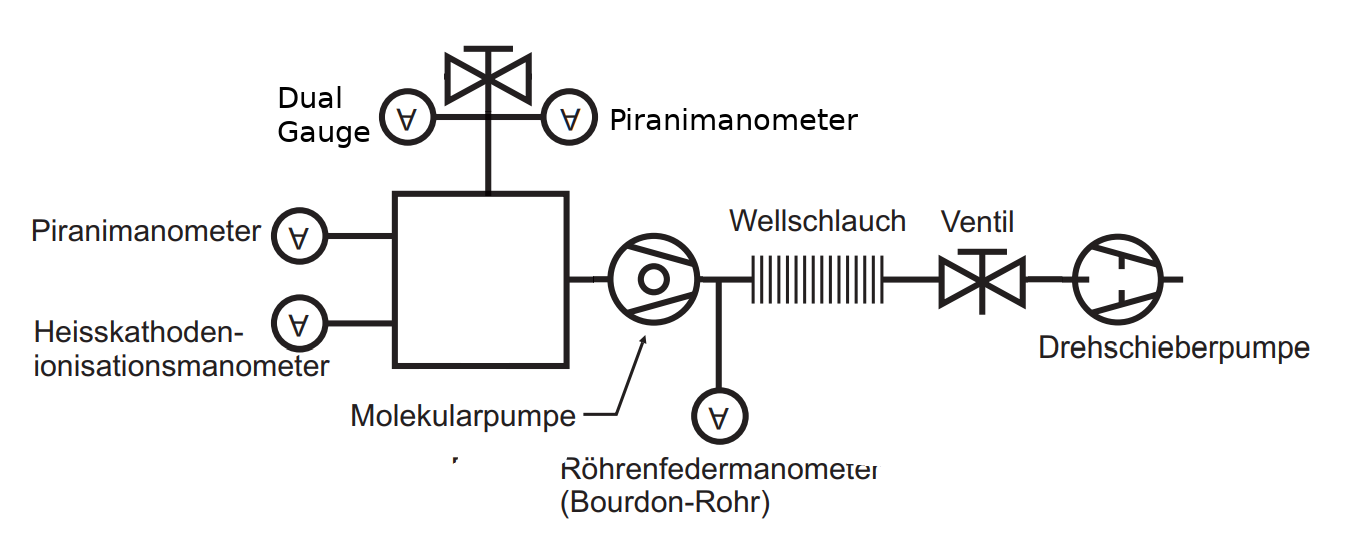
\includegraphics[width=.55\paperwidth]{aufbau24}
            \caption{Bestimmung des Saugvermögens einer TMP}
            \label{fig:anord4}
        \end{figure}
    
    	Es wird nun eine Kapillarröhre an den Rezipienten angeflanscht, diese hat ein Fassungsvolumen von 
        %TODO: $\ ml$
    
    	Mithilfe des Binärventils wird nun der gewünschte Druck eingestellt. Ein Seifentropfen wird in die Kapillare eingegeben und die Dauer gemessen, die der Tropfen benötigt um eine gewünschtes Volumen in der Kapillare zu überschreiten
    	
    	\begin{figure}[H]
    		\centering
    		\begin{tabular}{llll}
\toprule
                                   V / ml &                                     p / mbar &                                    t / s &                                       V / ml \\
\midrule
 $\left(1.00 \pm 0\right) \times 10^{-1}$ &  $\left(9.60 \pm 0.10\right) \times 10^{-6}$ &  $\left(3.31 \pm 0\right) \times 10^{1}$ &  $\left(3.00 \pm 0.10\right) \times 10^{-2}$ \\
 $\left(2.00 \pm 0\right) \times 10^{-1}$ &  $\left(2.90 \pm 0.10\right) \times 10^{-5}$ &  $\left(2.06 \pm 0\right) \times 10^{1}$ &  $\left(6.00 \pm 0.20\right) \times 10^{-2}$ \\
 $\left(2.00 \pm 0\right) \times 10^{-1}$ &  $\left(1.10 \pm 0.10\right) \times 10^{-4}$ &  $\left(5.73 \pm 0\right) \times 10^{0}$ &  $\left(6.00 \pm 0.20\right) \times 10^{-2}$ \\
 $\left(5.00 \pm 0\right) \times 10^{-1}$ &  $\left(2.90 \pm 0.10\right) \times 10^{-4}$ &  $\left(1.25 \pm 0\right) \times 10^{1}$ &  $\left(3.00 \pm 0.10\right) \times 10^{-1}$ \\
  $\left(1.00 \pm 0\right) \times 10^{0}$ &  $\left(1.10 \pm 0.10\right) \times 10^{-3}$ &  $\left(4.54 \pm 0\right) \times 10^{0}$ &  $\left(4.00 \pm 0.10\right) \times 10^{-1}$ \\
\bottomrule
\end{tabular}

            \caption{Messreihe 1.1 - Saugvermögen bei Kapillare 1}
    	\end{figure}
    	
    	Die Kapillare wurde nun durch eine Andere ersetzte, diese besitzt ein Fassungsvolumen von 
        %TODO: $\ ml$, 
        und es wurden folgende Messungen gemacht:
    	
 	    \begin{figure}[H]
    		\centering
    		\begin{tabular}{lll}
\toprule
                                    p / mbar &                                    t / s &                                      V / ml \\
\midrule
 $\left(1.10 \pm 0.10\right) \times 10^{-3}$ &  $\left(5.45 \pm 0\right) \times 10^{1}$ &  $\left(5.00 \pm 0.50\right) \times 10^{0}$ \\
 $\left(2.90 \pm 0.10\right) \times 10^{-4}$ &  $\left(6.10 \pm 0\right) \times 10^{1}$ &  $\left(2.00 \pm 0.50\right) \times 10^{0}$ \\
 $\left(3.10 \pm 0.10\right) \times 10^{-3}$ &  $\left(2.40 \pm 0\right) \times 10^{1}$ &  $\left(5.50 \pm 0.50\right) \times 10^{0}$ \\
 $\left(1.00 \pm 0.10\right) \times 10^{-2}$ &  $\left(1.71 \pm 0\right) \times 10^{1}$ &  $\left(1.00 \pm 0.05\right) \times 10^{1}$ \\
 $\left(3.40 \pm 0.10\right) \times 10^{-2}$ &  $\left(1.13 \pm 0\right) \times 10^{1}$ &  $\left(1.50 \pm 0.05\right) \times 10^{1}$ \\
\bottomrule
\end{tabular}

            \caption{Messreihe 1.2 - Saugvermögen bei Kapillare 2}
    	\end{figure}
    	
    	Es erfolgt eine weitere Kapillare mit dem Fassungsvermögen von $\ ml$, mit den folgenden Messungen:
    	
    	\begin{figure}[H]
			\centering
			\begin{tabular}{llll}
\toprule
Empty DataFrame
Columns: Index(['p / mbar', 't / s', 'V / ml'], dtype='object')
Index: RangeIndex(start=0, stop=0, step=1) \\
\bottomrule
\end{tabular}

            \caption{Messreihe 1.3 - Saugvermögen bei Kapillare 3}
		\end{figure}
    	
    	Zuletzt wird ein Kolben angebracht:
    	
    	\begin{itemize}
    		\item Gesamtvolumen: $(35\pm3)\ ml$ (Schätzung)
    		\item Masse: $m=44.67\ g$
    		\item Skalenteilung: $0.5\ ml$
            % 26.5mm/5ml
    		\item Durchmesser: $d=(15.5\pm0.1)\cdot10^{-3}\ m$
    	\end{itemize}
    
    	\begin{figure}[H]
			\centering
            \begin{tabular}{llll}
\toprule
Empty DataFrame
Columns: Index(['p / mbar', 't / s', 'V / ml'], dtype='object')
Index: RangeIndex(start=0, stop=0, step=1) \\
\bottomrule
\end{tabular}

			\caption{Messreihe 1.4 - Saugvermögen bei Kolben}
		\end{figure}
    	
    	(Diese Messungen geschehen bei Äußerem Normaldruck)
    	Anschließend wird langsam belüftet um die TMP nicht zu überhitzen
    	
    
    \subsection{Leitwert von Rohr und Blende}
    
        \begin{figure}[H]
            \centering
            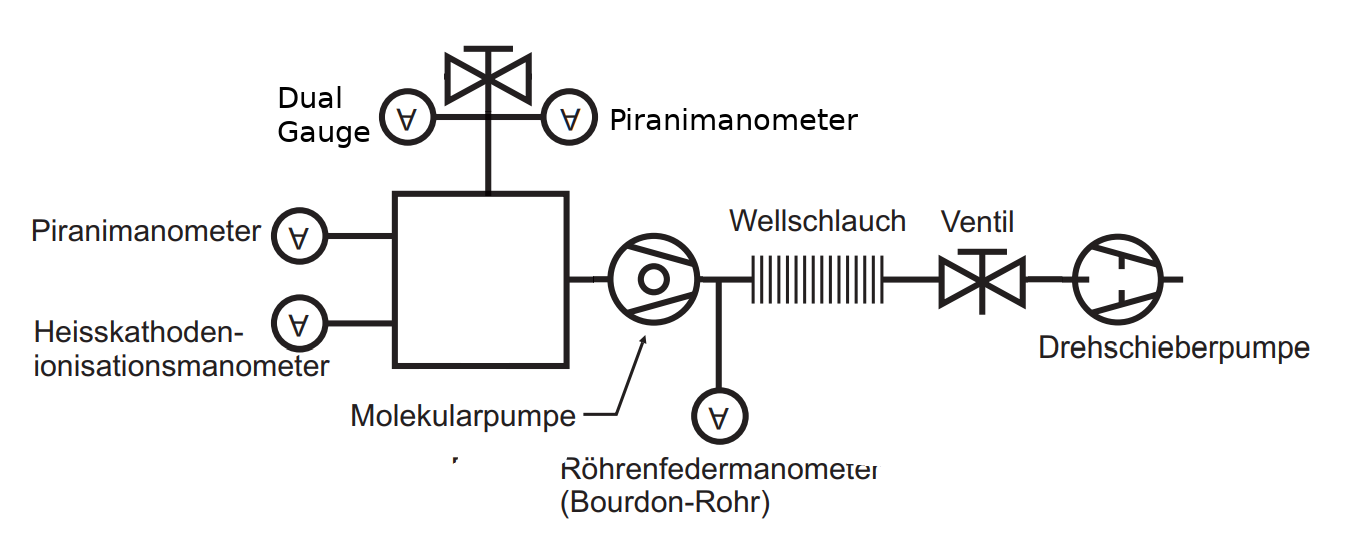
\includegraphics[width=.55\paperwidth]{aufbau24.png}
            \caption{Aufbau zur Bestimmung des Leitwerts von Rohr und Blende}
            \label{fig:anord5}
        \end{figure}
    
    	Der Rezipient wird nun leer gepumpt und anschließend mittels Binärventil der gewünschte Druck eingestellt. Bei verschiedenen Rohren und Blenden in der Führung wird der Druck jeweils oben am Führrohr und unten am Rezipienten gemessen (mithilfe der Dual-Gauge)
    	
    	\begin{itemize}
            %TODO
    		\item Maße Blende:
    			\begin{align*}
    				d=&(4.2\pm 0.1)\cdot 10^{-3}\ m\\
    				h=&(5.0\pm 0.1)\cdot 10^{-3}\ m
    			\end{align*}
    			
    		\item Maße Rohr:
    			\begin{align*}
    				d=&(12.0\pm 0.1)\cdot 10^{-3}\ m\\
    				h=&(1.00\pm 0.05)\cdot \ m
    			\end{align*}
    			
    		\item Maße Halterohr:
    			\begin{align*}
    				d=&(52.0\pm 0.1)\cdot 10^{-3}\ m\\
    				h=&(1.00\pm 0.05)\cdot \ m
    			\end{align*}
    	\end{itemize}
    
    	\begin{figure}[H]
    		\centering
    		\caption{Messreihe 2.1: Rohr und Blende}
    		%TODO: \begin{tabular}{ll}
\toprule
                                $p_o$ / mbar &                                 $p_u$ / mbar \\
\midrule
 $\left(5.80 \pm 0.10\right) \times 10^{-3}$ &  $\left(5.40 \pm 0.10\right) \times 10^{-5}$ \\
 $\left(2.40 \pm 0.10\right) \times 10^{-2}$ &  $\left(9.70 \pm 0.10\right) \times 10^{-5}$ \\
 $\left(4.40 \pm 0.10\right) \times 10^{-2}$ &  $\left(1.70 \pm 0.10\right) \times 10^{-4}$ \\
 $\left(7.10 \pm 0.10\right) \times 10^{-2}$ &  $\left(3.30 \pm 0.10\right) \times 10^{-4}$ \\
 $\left(9.50 \pm 0.10\right) \times 10^{-2}$ &  $\left(5.60 \pm 0.10\right) \times 10^{-4}$ \\
 $\left(1.30 \pm 0.10\right) \times 10^{-1}$ &  $\left(1.10 \pm 0.10\right) \times 10^{-3}$ \\
 $\left(1.80 \pm 0.10\right) \times 10^{-1}$ &  $\left(2.00 \pm 0.10\right) \times 10^{-3}$ \\
 $\left(2.20 \pm 0.10\right) \times 10^{-1}$ &  $\left(3.30 \pm 0.10\right) \times 10^{-3}$ \\
 $\left(2.60 \pm 0.10\right) \times 10^{-1}$ &  $\left(5.70 \pm 0.10\right) \times 10^{-3}$ \\
 $\left(3.20 \pm 0.10\right) \times 10^{-1}$ &  $\left(1.00 \pm 0.10\right) \times 10^{-2}$ \\
\bottomrule
\end{tabular}

   		\end{figure}
   	
   		Nach der Messung wird die Pumpe belüftet. Das Halterohr abgeschraubt und die Blende entfernt. Nach erneutem anbringen des Halterohrs wird erneut eine Druckmessung durchgeführt.
   	
   		\begin{figure}[H]
   			\centering
   			\caption{Messreihe 2.2: Rohr}
   			%TODO: \begin{tabular}{ll}
\toprule
                                $p_o$ / mbar &                                 $p_u$ / mbar \\
\midrule
 $\left(5.90 \pm 0.10\right) \times 10^{-3}$ &  $\left(5.50 \pm 0.10\right) \times 10^{-5}$ \\
 $\left(2.20 \pm 0.10\right) \times 10^{-2}$ &  $\left(1.00 \pm 0.10\right) \times 10^{-4}$ \\
 $\left(4.20 \pm 0.10\right) \times 10^{-2}$ &  $\left(1.80 \pm 0.10\right) \times 10^{-4}$ \\
 $\left(6.60 \pm 0.10\right) \times 10^{-2}$ &  $\left(3.40 \pm 0.10\right) \times 10^{-4}$ \\
 $\left(8.70 \pm 0.10\right) \times 10^{-2}$ &  $\left(5.50 \pm 0.10\right) \times 10^{-4}$ \\
 $\left(1.20 \pm 0.10\right) \times 10^{-1}$ &  $\left(1.00 \pm 0.10\right) \times 10^{-3}$ \\
 $\left(1.50 \pm 0.10\right) \times 10^{-1}$ &  $\left(1.80 \pm 0.10\right) \times 10^{-3}$ \\
 $\left(2.00 \pm 0.10\right) \times 10^{-1}$ &  $\left(3.20 \pm 0.10\right) \times 10^{-3}$ \\
 $\left(2.40 \pm 0.10\right) \times 10^{-1}$ &  $\left(5.60 \pm 0.10\right) \times 10^{-3}$ \\
 $\left(3.10 \pm 0.10\right) \times 10^{-1}$ &  $\left(1.10 \pm 0.10\right) \times 10^{-2}$ \\
\bottomrule
\end{tabular}

   		\end{figure}
   	
   		Die Pumpe wird belüftet und als letzte Messreihe lediglich die Blende in das Halterohr montiert. Der Rezipient wird erneut evakuiert und eine erneute Druckmessung durchgeführt.
   	
   		\begin{figure}[H]
   			\centering
   			\caption{Messreihe 2.3: Blende}
   			%TODO: \begin{tabular}{ll}
\toprule
                                $p_o$ / mbar &                                 $p_u$ / mbar \\
\midrule
 $\left(9.40 \pm 0.10\right) \times 10^{-4}$ &  $\left(5.60 \pm 0.10\right) \times 10^{-5}$ \\
 $\left(3.20 \pm 0.10\right) \times 10^{-3}$ &  $\left(9.80 \pm 0.10\right) \times 10^{-5}$ \\
 $\left(7.30 \pm 0.10\right) \times 10^{-3}$ &  $\left(1.80 \pm 0.10\right) \times 10^{-4}$ \\
 $\left(1.40 \pm 0.10\right) \times 10^{-2}$ &  $\left(3.20 \pm 0.10\right) \times 10^{-4}$ \\
 $\left(2.40 \pm 0.10\right) \times 10^{-2}$ &  $\left(5.60 \pm 0.10\right) \times 10^{-4}$ \\
 $\left(4.10 \pm 0.10\right) \times 10^{-2}$ &  $\left(1.00 \pm 0.10\right) \times 10^{-3}$ \\
 $\left(6.20 \pm 0.10\right) \times 10^{-2}$ &  $\left(1.90 \pm 0.10\right) \times 10^{-3}$ \\
 $\left(9.10 \pm 0.10\right) \times 10^{-2}$ &  $\left(3.30 \pm 0.10\right) \times 10^{-3}$ \\
 $\left(1.20 \pm 0.10\right) \times 10^{-1}$ &  $\left(5.40 \pm 0.10\right) \times 10^{-3}$ \\
 $\left(1.70 \pm 0.10\right) \times 10^{-1}$ &  $\left(1.00 \pm 0.10\right) \times 10^{-2}$ \\
\bottomrule
\end{tabular}

   		\end{figure}    
    
    
    \subsection{Lecksuche}
    
		Zunächst wird der Aufbau aus Versuchsteilen 4 \& 5 benutzt\\\\	
		$\rightarrow$ Über Nacht hat sich ein Druck von 
        $(3.6\pm0.1)\cdot 10^{-1}\ mbar$
        eingestellt.\\\\
		Die Pumpen werden erneut eingeschalten. Es wird ein aus Glas geschmolzenes Leck aus dem Auslass des Ventils am Rezipienten angebracht.\\
		$\rightarrow$ Mit dem Leck stellt sich ein Druck von 
        %TODO: $(\pm)\cdot 10^{}\ mbar$
        ein.\\		
		Die Strahlenkanone wurde dann auf die Glaskapillare gehalten.\\
		$\rightarrow$ Der Luftstrom war durch die Gasentladung sehr deutlich zu sehen.\\\\		
		Für die Gegenstromlecksuche wurde folgender Aufbau verwendet:
		
		\begin{figure}[H]
			\centering
			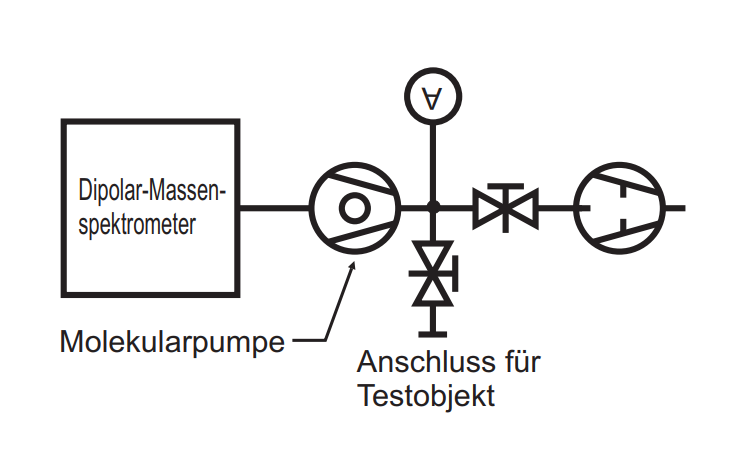
\includegraphics[width=.3\paperwidth]{aufbau262}
			\caption{Prinzipschaltbild des im Versuchsteil 6 eingesetzten Gegenstromlecksuchers}
			\label{fig:anord6}
		\end{figure}
		Mittels einer Heliumgasflasche wurde am verschiedenen Stellen Helium auf die Apparatur gegeben und der Ausschlag am Spektrometer beobachtet.\\
		$\rightarrow$ Es konnte eine poröse Schweißnaht ausfindig gemacht werden, die offensichtlich für das Leck im Aufbau verantwortlich ist.

	\section{Ergebnisse}
	\subsection{Inbetriebnahme der Drehschieberpumpe}
	
		Nach Inbetriebnahme der Drehschieberpumpe wurde der Druck im Rezipienten mittels des Dual-Gauge-Druckmessgerätes verfolgt.
		
		Nach kurzer Laufzeit der Pumpe wird die Druckveränderung mitverfolgt, dabei fällt der Druck innerhalb von 
        %TODO: $\ min
        auf 
        %TODO: $(\pm)\cdot 10^{-2}\ mbar$
        ab und verweilt dort für 
        %TODO: wieviele?
        weitere Minuten
		desshalt schätzen wir, dass der Enddruck bis auf
		\begin{align*}
            %TODO: pfffft
			p=(\pm)\cdot 10^{-2}\ mbar
		\end{align*}
		(Fehler ist Schätzung) fallen wird, auch wenn wir die Pumpe über mehrere Stunden Hinweg arbeiten lassen könnten.
		
		Das Vakuum kann mit einer Drehschieberpumpe nicht beliebig gut werden, da die Drehschieberpumpe bei einem gewissen Druck das Gas nicht mehr genügend komprimieren kann, was zum Ausstoßen des Gases nötig wäre.
		Es stellt sich aber ein Gleichgewicht bei einem bestimmten Druck ein, sodass die Menge an Gas, die von der Pumpe nach außen gefördert wird, gerade der Menge Gas entspricht, die durch Lecks, oder Pseudolecks in den Rezipienten eintritt.
		
		
	\subsection{Abpumpen kondensierbarer Dämpfe}
		
		\begin{figure}[H]
			\centering
			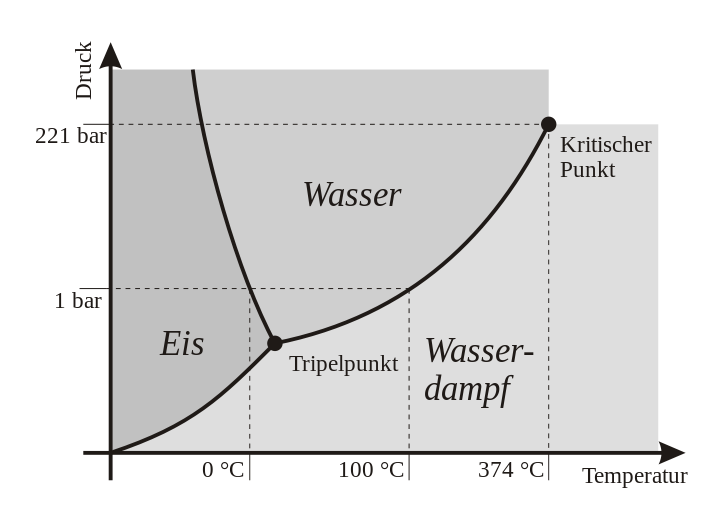
\includegraphics[width=.5\paperwidth]{phasen-wasser}
			\caption{Phasendiagramm von Wasser (nach \cite{wikibooks})}
		\end{figure}
    
        Im zweiten Teil des Versuchs konnten wir beobachten, wie Wasser verschiedene Zustände durchläuft:
        
        \begin{itemize}
            \item Das Wasser startet bei Normaldruck und Raumtemperatur
            
            \item Der Druck im Rezipienten fällt zu Beginn sehr stark, da die Pumpe eine große Gasmenge fördern kann. Die Temperatur des Wassers sollte dabei konstant bleiben. Ab einem Druck um $11\ mbar$ sollte das Wasser zu kochen beginnen.
            
            \item Durch das siedende Wasser und den entstehenden Wasserdampf kann die Drehschieberpumpe nicht weiter arbeiten\\
            $\rightarrow$ Das Gasballastventil wird geöffnet
            
            \item Die Pumpe kann nun weiter arbeiten und der Zustand des Wassers wandert entlang der Dampfdruckkurve
            
            \item bei etwa $(5.8\pm0.1)\ mbar$, gefriert das Wasser, da nun der Tripelpunkt überschritten ist\\(Literaturwert: $6\ mbar\ \rightarrow\ 2\sigma$)
        \end{itemize}

    \subsection{Inbetriebnahme einer TMP}
    
        Die TMP erreichte (nach einer Nacht) einen Druck von 
        %TODO: $(\pm 0.1)\cdot10^{-6}\ mbar$, 
        was den durch die Drehschieberpumpe errreichten Druck um 
        %TODO 
        Größenordnungen absenkt, was solange dauert da Gase im Rezipienten desorbieren (Pseudoleck)
        
    \subsection{Saugvermögen der TMP}
        
        Nach dem Anbringen der Kapillare stellt sich ein Gleichgewicht ein, das durch die Kapillare eingesaugte Luftvolumen $V6$ entspricht dann genau dem im Reipienten abgesaugten Volumen $V_R$ (pro Zeit):
        \begin{align}
            pV=nRT
        \end{align}
        (Druck p, Volumen V, Stoffmenge n, Gaskonstante R und Temperatur T)
        \begin{align}
            \frac{p_{außen}V}{t} =& \frac{p_{innen}V_R}{t}\\
            \Leftrightarrow S=&\frac{V_R}{t}=\frac{V_R}{t}\cdot \frac{p_{außen}}{p_{innen}}\\
            \Delta S=&\sqrt{
                (\frac{\Delta t}t)^2
                (\frac{\Delta V}V)^2
                (\frac{\Delta p_{innen}}{p_{innen}})^2
            }\cdot S
        \end{align}
	
        Auf den Fehler von $p_{außen}$ wurde verzichtet und es wurde der Literaturwert von $1013\ hPa$ verwendet.
        Die errechneten Wee für das Saugvermögen sind in Tabelle
        %TODO: ref
        zu finden, die Daten wurden zudem in Abbildung
        %TODO ref
        aufgetragen und ein linearer Fit durchgeführt
        
        \begin{figure}[H]
            \centering
            %TODO: tabelle 34-t1.tex?
            \caption{Tabelle der errechnete Werte des Saugvermögens}
        \end{figure}
    
        \begin{figure}[H]
            \centering
            %TODO: diagramm 34-f1.png?
            \caption{Messwerte des Saugvermögens einer TMP}
        \end{figure}
        
        \begin{align*}
            %TODO val
            S=(\pm)\ \frac{l}{s}
        \end{align*}
        
        \begin{itemize}
            \item Deutlich zu sehen ist, dass die mit dem Kolben gemessenen Werte systematisch zu hoch liegen. Dies liegt daran, dass der Kolben durch sein eigenes Gewicht noch zusätzlich Luftvon außen hereindrückt.
            
            \item Es war zudem ein recht poröser Schlauch am Kolben angebracht, der für ein größeres Leck sorgt und somit die Messung verfälscht.
            
            \item Fehler bei den Kapillaren können dadurch zustande gekommen sein, dass die Kapillare in ihrer Halterung leicht schräg war und nicht senkrecht. Der Tropfer erfuhr daher eine Hangabtriebskraft weg vom Rezipienten
        \end{itemize}
        Wie könnte man die Genauigkeit der Messung erhöhen?
        
        Zu Beginn bei sehr kleinem eingesaugten Volumen könnten noch dünnere Kapillare die zeitliche Genauigkeit erhöhen, da der Tropfen dann mit höherer Geschwindigkeit durch die Kapillare laufen würde.
    
    \subsection{Leitwert von Rohr und Blende}
    
        Bei verschiedenen eingebauten Teilen (Rohr, Blende) wurden die Druckdifferenzen oberhalb und unterhalb des Bauteils gemessen um den Leitwert des Aufbaus zu bestimmen. Mit dem in Teil 3 bestimmten Saugvermögen lässt sich über die Druckdifferenz $\delta p$ auf den Leitwert L schließen, mittels:
        
        \begin{align}
            L=&\frac{Q}{\delta p}
            \intertext{(Saugleistung Q)}
            \text{mit } Q=&S\cdot p_{unten}\\
            \Rightarrow L=&\frac{S\cdot p_{unten}}{\delta p}\\
            \delta p=& p_{oben} - p_{unten}
            \intertext{mit dem Fehler:}
            \Delta (\delta p) =& \sqrt{\Delta p_{oben}^2+ \Delta p_{unten}^2}\\
            \Delta L=&\sqrt{(\frac{\Delta S}S)^2+(\frac{\Delta p_{unten}}{p_{unten}})^2+(\frac{\Delta (\delta p)}{\delta p})^2}\cdot L
        \end{align}
        Die Berechnung für die 3 Konfigurationen aus Rohr und Blende sind in den Tabellen
        %TODO: ref
        zu finden
        
        \begin{figure}[H]
            \centering
            %TODO: \input{34-t1.tex}
            \caption{}
        \end{figure}
    
        \begin{figure}[H]
            \centering
            %TODO: \input{34-t2.tex}
            \caption{}
        \end{figure}
    
        \begin{figure}[H]
            \centering
            %TODO: \input{34-t3.tex}
            \caption{}
        \end{figure}
    
        Die Daten der Leitwerte sind in den Diagrammen
        %TODO: ref
        aufgetragen. zu sehen ist bei allen 3 Konfigurationen ein Anstieg des Leitwertes hin zu kleinen Drücken
        %TODO: ($p < 10^-4\ mbar$)
        und hin zu sehr großen Drücken.
        %TODO: ($p > 3\cdot 10^-3\ mbar$)
        Dies hat damit zu tun, dass in dieser Berechnung das Saugvermögen über den gesamten Druckbereich als konstant angenommen wurde. Wie in Diagramm
        %TODO: ref
        zu sehen, ist dies keinesfalls so.
        Der Leitwert ist in diesen Bereichen wegen des zu groß angenommenen Saugvermögens selbst auch viel zu hoch. Bei den hohen Drücken gibt es außerdem den Effekt, dass hier schon der Übergang von der molekularen Strömung zur laminaren Strömung kommt und der Leitwert damit ansteigt.
        Zur Bestimmung des Leitwerts im molekularen Bereich wurde daher ein Fit (konstant) an die Messpunkte im Bereich 
        %TODO: $2\cdot 10^{-4}$ bis $2\cdot 10^{-3}\ mbar$
        gemacht:
        
        \begin{align*}
            %TODO: val
            \text{Rohr: }L_R=&(\pm)\ \frac l s\\
            \text{Blende: } L_B=&(\pm)\ \frac l s\\
            \text{Rohr + Blende: } L_{R+B}=&(\pm)\ \frac l s
        \end{align*}
        
        \subsubsection*{Überprüfung der kirchhoffschen Regeln}
    
    \subsection{Lecksuche}
	
	\section{Diskussion}
    
    (Teil 5: Rohrdurchmesser zu groß gewählt?)
	
	Hier werden alle wesentlichen Ergebnisse nochmals ausgefuehrt und diskutiert. 
	
	Am Schluss kann man noch eine allgemeinere Bemerkung zum Versuch machen.
	
	
	\newpage 
	
	\begin{thebibliography}{00}   % {00}: max 2-stellig
		
		\bibitem{skript} Versuchsskript zu Versuch F70
		
		\bibitem{wikibooks} de.wikibooks.org: Aggregatszustandsänderungen\\ (\url{https://de.wikibooks.org/wiki/Physik_in_unserem_Leben/_Aggregatzustands%C3%A4nderungen})
		
	\end{thebibliography}
	
\end{document}